\subsection{Learnable Attention Mechanisms}
\label{sec:learnable-attention-mechanisms}

\subsubsection{Self-attention}

A way to use attention is called \textbf{self-attention}.
\[
    \tilde{X}=\text{softmax}_\text{row}(\frac{XX^T}{\sqrt{k}})X=\text{Attention}(X,X,X)=\text{SelfAttention}(X)
\]

We can see that:
\[
    XX^T=\begin{bmatrix}
    x_1x_1^T & x_1x_2^T & \ldots & x_1x_n^T\\
    x_2x_1^T & x_2x_2^T & \ldots & x_2x_n^T\\
    \vdots & \vdots & \ddots & \vdots\\
    x_nx_1^T & x_nx_2^T & \ldots & x_nx_n^T
    \end{bmatrix}
\]

So we are computing how much each word is similar to
every other word in the sentence.
We then use the softmaxed attention scores to compute the
weighted sum of the values (the same sentence).
So $\tilde{x}_1$ is going to be $\sum_{i=1}^{n}\alpha_ix_i$.
This process changes the embeddings for each word,
making it more appropriate for the context.

This process is still $O(n^2)$.

When we have a sentence that is generated with time,
at each time step we can "see" only the previous words.
How can we still parallelize this process if all the $X$ matrices
are different at each time step? (e.g. $X_1=[x_1], X_2=[x_1, x_2]$ etc.)
We want that each word computes its similarity only with 
previous words. How can we make the future words get an
attention score of $0$? We need to set the similarity to
$-\infty$ to make the softmax output $0$. To achieve this
we can set the upper triangular part of the matrix to $-\infty$.
Like this:
\[
    \frac{XX^T}{\sqrt{k}}+M=\begin{bmatrix}
        a_{11} && \ldots && a_{1n}\\
        \vdots && \ddots && \vdots\\
        a_{n1} && \ldots && a_{nn}
    \end{bmatrix} + \begin{bmatrix}
        0 & -\infty & \ldots & -\infty\\
        0 & 0 & \ldots & -\infty\\
        \vdots & \vdots & \ddots & \vdots\\
        0 & 0 & \ldots & 0
    \end{bmatrix}
\]

We call the matrix $M$ a \textbf{causal mask} and the operation is called \textbf{causal self-attention}.

\subsubsection{Attention head}

By default there's nothing that can learn in the attention mechanism.
Assume that we have a:
\begin{itemize}
    \item queries $Q$
    \item keys $K$
    \item values $V$
\end{itemize}
We can learn a projection for each of them.
So we compute:
\begin{itemize}
    \item $Q'=QW_Q$
    \item $K'=KW_K$
    \item $V'=VW_V$
\end{itemize}
Instead of computing the attention scores with $Q$ and $K$ we use $Q'$ and $K'$ and then
we use $V'$ to compute the weighted sum.
\[
    \tilde{V}=\text{softmax}_\text{row}(\frac{QW_q(KW_K)^T}{\sqrt{k}})VW_V
\]
Matrices $W_Q$, $W_K$ and $W_V$ do not need to be square, they can be of any size with the constraint
that $W_Q$ and $W_K$ go to the same output size.
\begin{figure}[H]
    \centering
    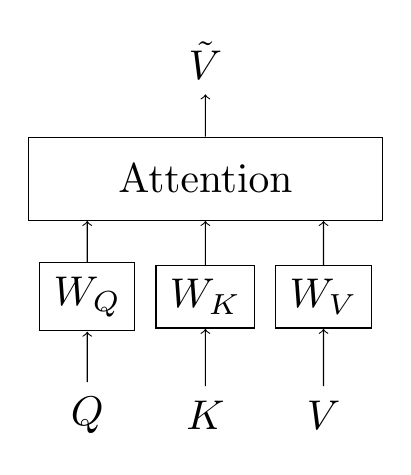
\begin{tikzpicture}[scale=1.5, every node/.style={scale=1.5}]
        % Nodes
        \node (K) {$K$};
        \node (Q) [left of=K] {$Q$};
        \node (V) [right of=K] {$V$};
        \node (W_K) [draw, rectangle, above of=K] {$W_K$};
        \node (W_Q) [draw, rectangle, above of=Q] {$W_Q$};
        \node (W_V) [draw, rectangle, above of=V] {$W_V$};
        \node (attention) [draw, rectangle, above of=W_K, minimum width=3cm, minimum height=0.7cm] {Attention};
        \node (output) [above of=attention] {$\tilde{V}$};

        % Arrows
        \draw [->] (Q) -- (W_Q);
        \draw [->] (K) -- (W_K);
        \draw [->] (V) -- (W_V);
        \draw [->] (W_Q) -- (W_Q.north |- attention.south);
        \draw [->] (W_K) -- (attention);
        \draw [->] (W_V) -- (W_V.north |- attention.south);
        \draw [->] (attention) -- (output);
    \end{tikzpicture}
    \caption{Attention Head}
    \label{fig:attention-head}
\end{figure}

This can be used as a layer in a neural network because it has learnable parameters.
The matrices $W_Q$, $W_K$ and $W_V$ learn how to project the queries, keys and values in compatible spaces.

\subsubsection{Multi-head attention}

Can we know if the learned projections are the best ones?
Of course not, but we can learn multiple different projections to be safe.

So instead of using a single attention head, we can use multiple attention heads.
Each of them is receiving the same input $Q,K,V$ and learns different projections.
So with $h$ heads we will have $h$ different outputs.
\[
    \tilde{V}=[\tilde{V}_1,\tilde{V}_2,\ldots,\tilde{V}_h]
\]
And then, with the concatenated output, we compute:
\[
    \tilde{\tilde{V}}=\tilde{V}W_O
\]
Where $W_O$ is a learnable matrix.

\begin{figure}[H]
    \centering
    \begin{tikzpicture}
        % Nodes
        \node (K) {$K$};
        \node (Q) [left of=K, node distance=0.5cm] {$Q$};
        \node (V) [right of=K, node distance=0.5cm] {$V$};
        \node (AH_1) [draw, rectangle, above of=K, minimum width=1.5cm] {$AH_1$};
        \node (AH_2) [draw, rectangle, right of=AH_1, node distance=2cm, minimum width=1.5cm] {$AH_2$};
        \node (AH_h) [draw, rectangle, right of=AH_2, node distance=2cm, minimum width=1.5cm] {$AH_h$};
        \node (concat) [draw, ellipse, above of=AH_1] {Concat};
        \node (W_O) [draw, rectangle, above of=concat] {$W_O$};
        \node (output) [above of=W_O] {$\tilde{\tilde{V}}$};

        % Arrows
        \draw [->] (Q) |- ++(0,0.5) -| (AH_1);
        \draw [->] (K) |- ++(0,0.5) -| (AH_1);
        \draw [->] (V) |- ++(0,0.5) -| (AH_1);
        \draw [->] (Q) |- ++(0,0.5) -| (AH_2);
        \draw [->] (V) |- ++(0,0.5) -| (AH_2);
        \draw [->] (K) |- ++(0,0.5) -| (AH_2);
        \draw [->] (Q) |- ++(0,0.5) -| (AH_h);
        \draw [->] (K) |- ++(0,0.5) -| (AH_h);
        \draw [->] (V) |- ++(0,0.5) -| (AH_h);
        \draw [->] (AH_1) |- ++(0,0.5) -| (concat);
        \draw [->] (AH_2) |- ++(0,0.5) -| (concat);
        \draw [->] (AH_h) |- ++(0,0.5) -| (concat);
        \draw [->] (concat) -- (W_O);
        \draw [->] (W_O) -- (output);
    \end{tikzpicture}
    \caption{Multi Head Attention}
    \label{fig:multi-head-attention}
\end{figure}

We can summarize the multi-head attention as:
\[
    \tilde{\tilde{V}}=MHA(Q,K,V|W_I,W_O)
\]
Summarizing all the input transformations for each head with $W_I$ and the output transformation with $W_O$.
We can use self attention and/or causal self attention in the multi-head attention.

\subsubsection{Training MHA}

We want to avoid two things:
\begin{itemize}
    \item Overfitting
    \item "Burning" neurons (neurons don't learn anything)
\end{itemize}

To avoid burning neurons we want to make the variance under control (to avoid exploding/vanishing gradients).
We want to avoid that in a single input there is a lot of variance.
To do this we don't apply batch normalization, but we use \textbf{layer normalization}.

If the input is $x\in\mathbb{R}^{1\times k}$ and the output is $y\in\mathbb{R}^{1\times k}$, we compute the layer normalization as:
\[
    y=\frac{x-\mu_x}{\sigma_x}
\]
Where $\mu_x=1/k\sum_{i=1}^{k}x_i$ and $\sigma_x=\sqrt{1/k\sum_{i=1}^{k}(x_i-\mu_x)^2 + \epsilon}$.
With $\epsilon$ a small number to avoid division by zero.

We can let this layer learn by adding two learnable parameters $\alpha$ and $\beta$:
\[
    \text{LayerNorm}(x|\alpha,\beta)=\alpha\frac{x-\mu_x}{\sigma_x}+\beta
\]

The second mechanism to avoid burning neurons is the \textbf{skip/residual connection}.

\begin{figure}[H]
    \centering
    \begin{tikzpicture}[scale=1.5, every node/.style={scale=1.5}]
        % Nodes
        \node (input) {$x$};
        \node (layer) [draw, rectangle, below of=input, node distance=1.2cm] {$F(x|W)$};
        \node (sum) [draw, ellipse, below of=layer, node distance=1cm] {$+$};
        \node (output) [below of=sum, node distance=1cm] {$y$};

        % Arrows
        \draw [->] (input) -- (layer);
        \draw [->] (layer) -- (sum);
        \draw [->] (sum) -- (output);
        \draw [->] (input) -- ++(0,-0.5) -| ++(1,-1) |- (sum);
    \end{tikzpicture}
    \caption{Skip Connection}
    \label{fig:skip-connection}
\end{figure}

When using residual connections we risk having a huge variance in the earlier layers, to avoid this
we never use residual without a normalization mechanism like layer normalization.
